\documentclass[Screen16to9,17pt]{foils}
\usepackage{zencurity-slides}

\usepackage{tabularx}
\usepackage{tikz}
\usetikzlibrary{mindmap,trees}
\usetikzlibrary{shapes.geometric, arrows,automata}
\usetikzlibrary{positioning}

\usepackage{jigsaw}



\tikzset{
    state/.style={
           rectangle,
           rounded corners,
           draw=black, very thick,
           minimum height=2em,
           inner sep=2pt,
           text centered,
           },
}


% Email Security - domains, clients and servers

% This presentation will be focused on email security overall - from domains to clients to servers. The presentation will include a lot of acronyms and some technical details, the goal though is to get an overview of available technologies and their benefits.

% We will talk about domains and the current internet standards and recommendations for setting DNS records and features to optimise the reception of email securely - using encryption and certificates. Also which DNS records and features will prevent your domains from being abused for sending fake emails such as phishing with you as the sender.

% We will discuss client features which are considered dangerous, loading images automatically etc. and how to improve your client security by using only specific protocols with encryption.

% Servers will be discussed as examples of email architectures. Common blueprints for email will be discussed including which components are to be used for getting insights into your email security - reporting functions. Example open source software will be shown.

% The goal for this presentation is for participants to get an overview of current email security, to allow them to evaluate their own posture - and plan a strategy to improve email security, both personally and professionally.

% Keywords: SMTP, TLS, DNS MX, DNS TXT, DMARC, SPF, DKIM, SMTP DANE - RFC 7672, MTA Strict Transport Security (MTA-STS), SMTP TLS Reporting, OpenARC, DMARC reporting, Postfix, Dovecot, Lets Encrypt certificates and Open Source mail tools

% Note: This presentation will not cover much filtering of anti-virus, phishing and malware except recommend having incoming and outgoing proxy servers where such services can be provided.

% Slides will be in english, but presentation language danish.


% Måske medtage Tyklings email IP source tip!



\begin{document}
\selectlanguage{danish}
\mytitlepage{Email Security - domains, clients and servers}{2020}


\slide{Goal for today}

\hlkimage{5cm}{Shaking-hands_web.jpg}

This presentation will be focused on email security overall - from domains to clients to servers. The presentation will include a lot of acronyms and some technical details, the goal though is to get an overview of available technologies and their benefits.




\begin{list2}
\item Plan:
\item Approx 4h, with breaks
\item Inspiration for solving the tasks, prioritizing the tasks
\item I dont have tailer made solutions or easy answers for your organisation
\end{list2}

\slide{Todays Agenda - approximate time plan}

\begin{list2}
\item[\faClockO] 17:00 - 18:15 Part I: Client Security and Email Threats
\item 30min Break - eat, drink and socialize
\item[\faClockO] 18:45 - 19:30 Part II: Basic Email Services
\item 15min break
\item[\faClockO] 19:45 - 20:15 Part III: Testing Email Services
\item 15min break
\item[\faClockO] 20:30 - 21:00 Part IV: Strategy for Your Email Security
\end{list2}

Please help me keep the time, thank you \smiley


\slide{Paranoia defined}

\hlkimage{12cm}{paranoia-definition.png}

Source: google paranoia definition


\slide{Hackers don't give a shit}

\hlkrightpic{10cm}{-2cm}{kiwicon-2009-hackers-dont-give-shit.jpg}

Your system is only for testing, development, ...

Your network is a research network, under construction, \\
being phased out, ...

Try something new, go to your management

Bring all the exceptions, all of them, update the risk \\
analysis figures - if this happens it is about 1mill DKK

Ask for permission to go full monty on your security

{\bf Think like attackers - don't hold back}


\slide{Confidentiality Integrity Availability}

\hlkimage{8cm}{cia-triad-uk.pdf}

\begin{list1}
\item We want to protect something
\item Confidentiality - data is kept confidential, secrets are secrets
\item Integrity - data is not subjected to unauthorized changes
\item Availability - data and systems are available for authorized users when they need it
\end{list1}


\slide{Overlapping Security Incidents}

\hlkrightpic{10cm}{1cm}{datalaek-2019.png}

New data breaches nearly every week, these from danish news site \link{version2.dk}

Problem, we need to receive data from others

Data from others may contain malware

Have a job posting, yes\\
- then HR will be expecting CVs sent as .doc and .pdf files

\slide{Part I: Client Security and Email Threats}

\hlkimage{6cm}{brian-patrick-tagalog-680954-unsplash.jpg}

We will discuss client features which are considered dangerous, loading images automatically etc. and how to improve your client security by using only specific protocols with encryption.



\slide{Attacking Email}

%\hlkrightpic{8cm}{-2cm}{brian-patrick-tagalog-680954-unsplash.jpg}
%{~}

\begin{list2}
\item Vi er afhængige af email, modtagelse og afsendelse
\item Når vi modtager skal det helst gå hurtigt
\item Når vi sender skal vi ikke ende i spam mappen
\item Phishing, hvem kan sende \emph{fra vores domæne}
\end{list2}


\slide{Various key attack types, clients and employees}

Attacking Email
\begin{list2}
\item Phishing - sending fake emails, to collect credentials
\item Spear phishing - targetted attacks
\item Person in the middle - sniffing and changing data in transit
\item Drive-by attacks - web pages infected with malware, often ad servers
\item Malware transferred via USB or email
\item Credential Stuffing, Password related, like re-use of password, see slide about being pwned
\end{list2}

\vskip 1cm
\centerline{\Large\bf If we all wait a bit, and not click links immediately}

\vskip 1cm
Hackers try to create "urgency", click this or loose money


\slide{The Internet Worm 2. nov 1988}

\begin{list1}
\item Exploited the following vulnerabilities
\begin{list2}
\item buffer overflow in fingerd - VAX code
\item Sendmail - DEBUG functionality
\item Trust between systems: rsh, rexec, ...
\item Bad passwords
\end{list2}
\item Contained camouflage!
\begin{list2}
\item Program name set to 'sh'
\item Used fork() to switch PID regularly
\item Password cracking using intern list of 432 words and /usr/dict/words
\item Found systems to infect in /etc/hosts.equiv, .rhosts, .forward, netstat ...
\end{list2}
\item Made byRobert T. Morris, Jr.
\end{list1}



\slide{Computer Viruses}

\begin{list1}
\item {\bf Definition 23-4} A \emph{computer virus} is a program that inserts (a possibly transformed version of) itself into one or more files and then performs some (possibly null) action.
\item Would spread through floppy disks and boot sector
\item Today more virus are spread through network shares, networked file systems
\begin{list2}
\item Boot sector virus - when booting a PC infects
\item A executable - exe files, similar types on PC platform .scr screensavers, .vbs visual basic scripts etc. Linux shell archives shar files.
\item Data - macro virus, found in Microsoft Office formats .doc etc.
\end{list2}
\item Polymorphic virus change their fingerprint/code during execution/infection
\item Definition from \emph{Computer Security: Art and Science}, 2nd ed, Matt Bishop, 2019
\end{list1}


\slide{Computer worms}

\begin{list1}
\item {\bf Definition 23-14} A \emph{computer worm} is a program that copies itself from one computer to another.
\item Definition from \emph{Computer Security: Art and Science}, 2nd ed, Matt Bishop, 2019
\item Computer worms has existed since research began mid-1970s
\item Morris Worm from November 2, 1988 was a famous example
\item ILOVEYOU worm from May 2000 written in Visual Basic was another
\vskip 2cm
\item Virus, trojan or worm?\\
Unless you work specifically in the computer virus industry, call it all malware

\end{list1}



\slide{Trojan horses}

\begin{list1}
\item {\bf Definition 23-1} \emph{Malicious logic}, more commonly called \emph{malware}, is a set\\
 of instructions that cause a site's security policy to be violated.
\item {\bf Definition 23-2} A \emph{Trojan horse} is a program with an overt (documented or\\
known) purpose and a covert (undocumented or unexpected) purpose.
\item Definitions from \emph{Computer Security: Art and Science}, 2nd ed, Matt Bishop, 2019
\item Book also mentions the Ken Thompson example with login program and compiler\\Insert Login backdoor, by inserting backdoor to notice when compiling compiler \smiley
\item Lots of free applications on Android have been trojans, for example stealing data
\end{list1}

The history lesson
\url{https://en.wikipedia.org/wiki/Trojan_Horse}\\
\url{https://en.wikipedia.org/wiki/Trojan_horse_(computing)}

\slide{Ransomware}


\begin{list1}
\item {\bf Defition 23-21} \emph{Ransomware} is malware that inhibits the use of resources until a ransom usually monetary, is paid.
\item Definition from \emph{Computer Security: Art and Science}, 2nd ed, Matt Bishop, 2019
\item Book also mentions 1989 example, PC CYBORG targetting PC/DOS computers
\item Uses cryptography to render data unreadable
\item Has become a huge problem for enterprises during the last 5-10 years
\item Often uses crypto-currencies today, like BitCoin (BTC) for payment
\item Often contains errors so decryption is impossible, or possible without payment!

\end{list1}


\slide{Phishing and spear phishing}


\begin{list1}
\item {\bf Definition 23-22} \emph{Phishing} is the act of impersonating a legitimate entity, typically a website associated with a business, in order to obtain information such as passwords, credit card numbers, and other private information without authorization
\item Example creating a fake bank website and make customers try to login
\item {\bf Definition 23-23} \emph{Spearphishing} is a phishing attack tailored for a particular victim.
\item Definitions from \emph{Computer Security: Art and Science}, 2nd ed, Matt Bishop, 2019
\end{list1}

\slide{Spear phishing -- targeted attacks}


Spearphishing - targeted attacks directed at specific individuals or companies

\begin{list2}
\item Use 0-day vulnerabilities only in a few places
\item Create backdoors and mangle them until not recognized by Anti-virus software
\item Research and send to those most likely to activate program, open file, visit page
\item Stuxnet is an example of a targeted attack using multiple 0-day vulns
\end{list2}

{\bf  A lot of threats are delivered through email or links sent via email}

also, we haven't solved email security problems in +30 years, and probably never will


\slide{Malware defenses}


\begin{list1}
\item {\bf Theorem 23.2} It is undecidable whether an arbitrary program contains a malicious logic.
\item Scanning defenses,
\begin{list2}
\item Check disk and memory for known bad malware signatures
\item Check for changes - integrity protection
\end{list2}
\item Behavioural - what does a malware do, that normal programs dont
\item Static analysis - what does a program normally do, what actions does malware do
\item Containment - change the environment to be more restricted
\item Theorem from \emph{Computer Security: Art and Science}, 2nd ed, Matt Bishop, 2019
\end{list1}

\vskip 1cm
\centerline{\bf \Large I dont trust or use anti-virus programs, fight me}

\slide{Vulnerabilities in popular mail programs}

\begin{list2}
\item They load pictures from the internet, enables tracking bugs\\
Disable as many features as possible, use a firewall
\item Show HTML, run JavaScript, run in browsers often - XSS Cross-site scripting\\
Decide if you trust browser or email client
\item Send headers with their specific version, enabling better buffer overflow attacks\\
Disable in mail client, and update often\\
{\bf All software has vulnerabilities}
\item Reveal IP - by connecting to server directly over internet\\
Only countermeasure might be to use VPN or Tor unless you run your own mail server
\item Allow cleartext authentication and sending, enabling snooping\\
Check your settings for using encrypting protocols TLS/STARTTLS
\item Also marks emails with sending date and time\\
How paranoid are you? Cases in Denmark regarding Snowden plane was \emph{interesting}
\end{list2}



\slide{Simple Mail Transfer Protocol (SMTP)}

\begin{quote}
  The Simple Mail Transfer Protocol (SMTP) is a communication protocol for electronic mail transmission. As an Internet standard, SMTP was first defined in 1982 by RFC 821, and updated in 2008 by RFC 5321 to Extended SMTP additions, which is the protocol variety in widespread use today. Mail servers and other message transfer agents use SMTP to send and receive mail messages.
\end{quote}

\url{https://en.wikipedia.org/wiki/Simple_Mail_Transfer_Protocol}


\slide{SMTP Simple Mail Transfer Protocol}

\begin{alltt}\tiny
hlk@bigfoot:hlk$ telnet mail.kramse.dk 25
Connected to sunny.
220 sunny.kramse.dk ESMTP Postfix
HELO bigfoot
250 sunny.kramse.dk
MAIL FROM: Henrik
250 Ok
RCPT TO: hlk@kramse.dk
250 Ok
DATA
354 End data with <CR><LF>.<CR><LF>
hejsa
.
250 Ok: queued as 749193BD2
QUIT
221 Bye
\end{alltt}

\begin{list2}
\item RFC-821 SMTP Simple Mail Transfer Protocol fra 1982
\item \link{http://en.wikipedia.org/wiki/Simple_Mail_Transfer_Protocol}
\end{list2}


\slide{Internet Message Access Protocol (IMAP)}

\begin{quote}
In computing, the Internet Message Access Protocol (IMAP) is an Internet standard protocol used by email clients to retrieve email messages from a mail server over a TCP/IP connection.[1] IMAP is defined by RFC 3501.

IMAP was designed with the goal of permitting complete management of an email box by multiple email clients, therefore clients generally leave messages on the server until the user explicitly deletes them. An IMAP server typically listens on port number 143. IMAP over SSL (IMAPS) is assigned the port number 993.

Virtually all modern e-mail clients and servers support IMAP, which along with the earlier POP3 (Post Office Protocol) are the two most prevalent standard protocols for email retrieval.[2] Many webmail service providers such as Gmail, Outlook.com and Yahoo! Mail also provide support for both IMAP and POP3.
\end{quote}

\url{https://en.wikipedia.org/wiki/Internet_Message_Access_Protocol}




\slide{Example of SMTP and IMAP}

\begin{center}
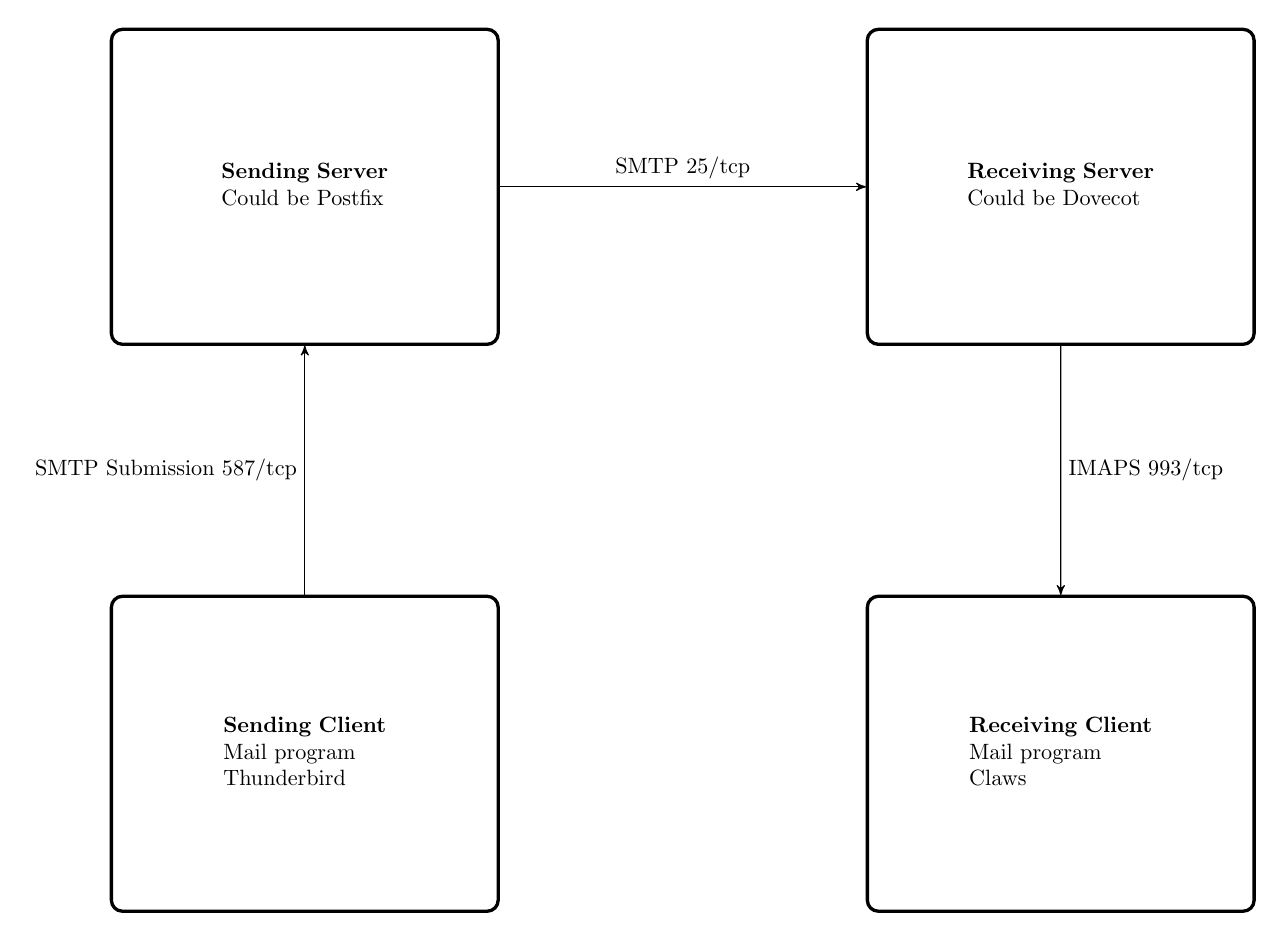
\begin{tikzpicture}[->,>=stealth',scale=0.8, transform shape]
  \newlength{\boxwidth}
  \setlength{\boxwidth}{6cm}
  \newlength{\boxheight}
  \setlength{\boxheight}{5cm}
  \newlength{\boxspace}
  \setlength{\boxspace}{12cm}

  % http://texample.net/tikz/examples/epc-flow-charts/

  % https://www.overleaf.com/learn/latex/LaTeX_Graphics_using_TikZ:_A_Tutorial_for_Beginners_(Part_3)%E2%80%94Creating_Flowcharts

   % Use previously defined 'state' as layout (see above)
   % use tabular for content to get columns/rows
   % parbox to limit width of the listing
   \node[state,text width=\boxwidth,minimum height=\boxheight] (SENDER)
   {\begin{tabular}{l}
   {\bf Sending Server}\\
      Could be Postfix
   \end{tabular}};

   %
   \node[state,         % layout (defined above)
    text width=\boxwidth,       % max text width
    minimum height=\boxheight,
    %yshift=2cm,                % move 2cm in y
    right of=SENDER,    % Position is to the right of QUERY
    node distance=\boxspace,    % distance to First node
    anchor=center] (RECEIVER)   % posistion relative to the center of the 'box'
   {%
   \begin{tabular}{l}
   {\bf Receiving Server}\\
Could be Dovecot
   \end{tabular}};

   \node[state,
    below of=SENDER,
    yshift=-8cm,
    anchor=center,
    minimum height=\boxheight,
    text width=\boxwidth] (THUNDERBIRD)
   {%
   \begin{tabular}{l}
   {\bf Sending Client}\\
    Mail program\\
    Thunderbird
   \end{tabular}
   };

   \node[state,
    below of=RECEIVER,
    yshift=-8cm,
    anchor=center,
    minimum height=\boxheight,
    text width=\boxwidth] (CLAWS)
   {%
   \begin{tabular}{l}
   {\bf Receiving Client}\\
    Mail program\\
    Claws
   \end{tabular}
   };
   % draw the paths and and print some Text below/above the graph
   \path
   (SENDER)     edge node[anchor=north,above]{SMTP 25/tcp} (RECEIVER)
   (THUNDERBIRD)        edge node[anchor=west,left]{SMTP Submission 587/tcp} (SENDER)
   (RECEIVER) edge node[anchor=east,right]{IMAPS 993/tcp }   (CLAWS);

\end{tikzpicture}
\end{center}



\slide{Securing Your Email Client}

\hlkimage{10cm}{thunderbird-enigmail-logo.png}

\begin{list2}
\item Security settings
\item Use TLS for SMTP
\item Use TLS for IMAPS
\item Disable loading of remote content, images, HTML parts, content, bugs, tracking
\item Disable sending version strings
\item Add plugins you need, but only those!
\end{list2}

Thunderbird mentioned as being one of the most popular email clients

\slide{Thunderbird Default Port Settings}

\hlkimage{16cm}{thunderbird-default-ports-auto.png}

By default Thunderbird will try to probe settings, which is fine

\slide{Thunderbird Chosen Port Settings}

\hlkimage{16cm}{thunderbird-default-ports-chosen.png}

I prefer to fix the ports to my known ports. Here running on default ports 993/tcp and 587/tcp

\slide{Inside an email -- headers}

\begin{alltt}\footnotesize
Return-Path: <hkj@zencurity.com>
X-Original-To: test@pentest.dk
Delivered-To: test@kramse.org{\bf
Received: from localhost (unknown [94.18.243.144])}
	(using {\bf TLSv1.2 with cipher ECDHE-RSA-AES256-GCM-SHA384 (256/256 bits))}
	(No client certificate requested)
	by mail.kramse.org ({\bf Postfix}) with ESMTPSA id 95958393EF
	for <test@pentest.dk>; Tue, 10 Mar 2020 15:05:05 +0100 (CET){\bf
Date: Tue, 10 Mar 2020 15:05:03 +0100}
From: Henrik Kramselund   <hkj@zencurity.com>
To: test@pentest.dk
Subject: Claws to Thunderbird
Message-ID: <20200310150503.7432a7a1@zencurity.com>
Organization: Zencurity Aps
MIME-Version: 1.0
Content-Type: text/plain; charset=UTF-8
Content-Transfer-Encoding: quoted-printable

--=20
Mvh/Best regards

Henrik
\end{alltt}

\slide{Thunderbird Default header User-Agent}

\begin{alltt}\footnotesize
To: hlk@kramse.org
From: Test <test@pentest.dk>
Subject: test headers
Message-ID: <25d9b367-872e-2858-b1ad-5c19a418bc54@pentest.dk>
Date: Tue, 10 Mar 2020 15:11:02 +0100{\bf
User-Agent: Mozilla/5.0 (X11; Linux x86_64; rv:68.0) Gecko/20100101
 Thunderbird/68.5.0}
MIME-Version: 1.0
Content-Type: text/plain; charset=utf-8; format=flowed
Content-Transfer-Encoding: 7bit
Content-Language: en-US

Almost empty email
\end{alltt}

So an attacker can now wait for a vulnerability in this \emph{specific version} and  \emph{specific operating system} -- Linux

\slide{CVE Details -- All software has errors! }
\hlkimage{19cm}{thunderbird-cves.png}

Source: {\footnotesize\url{https://www.cvedetails.com/product/3678/Mozilla-Thunderbird.html?vendor_id=452}}


\slide{Thunderbird Settings: }

\begin{quote}
Email messages can contain remote content such as images or stylesheets. To protect your privacy, Thunderbird does not load remote content automatically, but instead shows a notification bar to indicate that it blocked remote content.
\end{quote}

\begin{list2}
\item Privacy and security settings\\{\footnotesize \url{https://support.mozilla.org/da/products/thunderbird/privacy-and-security-settings}\\
\url{https://support.mozilla.org/en-US/products/thunderbird/privacy-and-security-settings}}
\item Previously you could override the User-Agent setting, setting it empty:\\
Does not work anymore
\url{https://bugzilla.mozilla.org/show_bug.cgi?id=1114475}
\item GPG and Enigmail for OpenPGP suppoprt - encrypted email\\
\url{https://support.mozilla.org/en-US/kb/digitally-signing-and-encrypting-messages}
\end{list2}

\slide{Claws Security Settings}

In my mail application there are other settings you can play with:

\begin{list2}
\item[\faCheck] Render HTML messages as text
\item[\faCheck] Use secure file deletion if possible
\item[\faCheck] Never send Return Receipts\\
When you receive a message that requests a Return Receipt a notification area is shown just above the message view. You can either use the 'Send receipt' button, or ignore the request - no receipts are sent automatically.
\item[\faSquareO] Automatically display attached images
\item[\faSquareO] Display images inline
\item[\faSquareO] Add user agent header -- don't
\end{list2}

BTW my mail client is not perfect either:\\{\footnotesize
\url{https://www.cvedetails.com/vulnerability-list/vendor_id-12415/Claws-mail.html}}

\slide{Other Email Clients}

\hlkrightpic{7cm}{-45mm}{google-email-pics.png}
{~}

\begin{list2}
\item Security settings Gmail
\item Good thing -- Scan your email for suspicious pictures, ask before loading
\item Bad thing for privacy -- they scan your email for commercial gain
\end{list2}

%\slide{Gmail Account Character Limit 12}

%\hlkrightpic{8cm}{-45mm}{google-12-chars.png}
%{~}

%{\Large\bf Why Google, why?!}

%Why in 2020 limit my password to 12 chars

\slide{Advanced: Run your mail client in a VM}

\hlkimage{10cm}{claws-email.png}

I run my email client in a VM, which can only connect to my mail server and my printer

\begin{alltt}\footnotesize
[hlk@dom0 ~]$ qvm-firewall Mailreader
NO  ACTION  HOST             PROTOCOL  PORT(S)  SPECIAL TARGET  ICMP TYPE  EXPIRE  COMMENT
0   accept  91.102.91.22/32  tcp       993      -               -          -       -
1   accept  91.102.91.22/32  tcp       587      -               -          -       -
2   accept  10.0.42.13/32    tcp       515      -               -          -       -
3   drop    -                -         -        -               -          -       -
[hlk@dom0 ~]$
\end{alltt}


\slide{Part II: Basic Email Services}

We will talk about domains and the current internet standards and recommendations for setting DNS records and features to optimise the reception of email securely - using encryption and certificates. Also which DNS records and features will prevent your domains from being abused for sending fake emails such as phishing with you as the sender.

Servers will be discussed as examples of email architectures. Common blueprints for email will be discussed including which components are to be used for getting insights into your email security - reporting functions. Example open source software will be shown.


\slide{Email Software}

My recommendations are:
\begin{list2}
\item Sending mail with SMTP using Postfix
\item Receiving mail with IMAP using Dovecot
\end{list2}

I would NOT use these:
\begin{list2}
\item Exim - multiple Remote Code Execution in 2019, fatal security vulns \\
\url{https://www.exim.org/static/doc/security/}
\item OpenSMTPD has had some really strange vulnerabilities recently\\
\url{https://www.opensmtpd.org/security.html}
\item Dont use Sendmail - old and horrible
\end{list2}


Many more exist: \url{https://en.wikipedia.org/wiki/Comparison_of_mail_servers}

\slide{Postfix}

\hlkimage{3cm}{postfix-mouse.png}

\begin{quote}\footnotesize
  Postfix is a free and open-source mail transfer agent (MTA) that routes and delivers electronic mail.

It is released under the IBM Public License 1.0 which is a free software license. Alternatively, starting with version 3.2.5, it is available under the Eclipse Public License 2.0 at the user's option.[2]

Originally written in 1997 by Wietse Venema at the IBM Thomas J. Watson Research Center in New York, and first released in December 1998[3], Postfix continues as of 2020 to be actively developed by its creator and other contributors.
\end{quote}
Source: \url{https://en.wikipedia.org/wiki/Postfix_(software)}

Home page: \url{http://www.postfix.org/}


\slide{Dovecot}

\begin{quote}\footnotesize
Dovecot is an open-source IMAP and POP3 server for Unix-like operating systems, written primarily with security in mind.[3] Timo Sirainen originated Dovecot and first released it in July 2002. Dovecot developers primarily aim to produce a lightweight, fast and easy-to-set-up open-source email server.

The primary purpose of Dovecot is to act as mail storage server. Mail is delivered to the server using some mail delivery agent (MDA) and stored for later access with an email client (mail user agent, or MUA).
\end{quote}
Source: \url{https://en.wikipedia.org/wiki/Dovecot_(software)}

\begin{quote}\footnotesize
Dovecot is an open source IMAP and POP3 email server for Linux/UNIX-like systems, written with security primarily in mind. Dovecot is an excellent choice for both small and large installations. It's fast, simple to set up, requires no special administration and it uses very little memory.
\end{quote}
Home page: \url{https://www.dovecot.org/}


\slide{Advanced: Removed headers -- client IP }

\hlkimage{18cm}{tykling-blog-email-privacy.png}

\url{https://blog.tyk.nu/blog/postfix-and-privacy/} Thank you Thomas


\slide{Internet i dag}

\hlkimage{10cm}{images/server-client.pdf}

\begin{list1}
\item Klienter og servere
\item Rødder i akademiske miljøer
\item Protokoller der er op til 20 år gamle
\item Meget lidt kryptering, mest på http til brug ved e-handel
\end{list1}



\slide{Data found in Network traffic }

\begin{list1}
\item Many older internet protocols are cleartext - no encryption
\item Lets take an example, DNS
\item Domain Name System DNS breadcrumbs
\begin{list2}
\item Your company domain, mail servers
\item Emails being sent are essentially post cards
\end{list2}
\vskip 1cm
\item Advice show your users, ask them to participate in a experiment
\item Sniffing a wireless network is easy
\end{list1}

\vskip 2 cm
\centerline{\bf\Large Maybe use VPN more - or always!}



\slide{Domain Name System}

\hlkimage{10cm}{dns-1.pdf}

\begin{list1}
\item Gennem DHCP får man typisk også information om DNS servere
\item En DNS server kan slå navne, domæner og adresser op
\item Foregår via query og response med datatyper kaldet resource records
\item DNS er en distribueret database, så opslag kan resultere i flere opslag
\end{list1}


\slide{DNS more than just web site name lookup}

% DNS MX, DNS TXT

\begin{list1}
  \item DNS is based on resource records of types:
    \begin{list2}
\item A-record is an address
\item Quad-A AAAA-records are IP version 6 addresses
\item Authoritative name servers are listed in NS-records
\item Email exchangers are put into MX-records
\item Multiple others: md ,  mf ,  cname ,  soa ,
                  mb , mg ,  mr ,  null ,  wks ,  ptr ,
                  hinfo ,  minfo ,  mx ....
\item Previously there was SRV server records and types being added, but today a lot of functionality is put into TXT records -- a text string with information
\end{list2}
\end{list1}

\begin{alltt}
ns1     IN      A       185.129.60.130
        IN      AAAA    2a06:d380:0:3065::53
www     IN      A       185.129.60.130
        IN      AAAA    2a06:d380:0:3065::80
\end{alltt}

\slide{DNS Example}


\begin{alltt}
user@Projects:images$ host -t ns zencurity.com
zencurity.com name server ns1.gratisdns.dk.
zencurity.com name server ns2.gratisdns.dk.
zencurity.com name server ns3.gratisdns.dk.
zencurity.com name server ns4.gratisdns.dk.
zencurity.com name server ns5.gratisdns.dk.
user@Projects:images$ host -t mx zencurity.com
zencurity.com mail is handled by 10 mail.kramse.org.
\end{alltt}

So this domain is found at the GratisDNS system and uses a single mail server record.

By default all of this happens without encryption and no integrity protection!

Note: I use mostly \verb+host+ while DNS admins typically use \verb+dig+

\slide{Well-known port numbers}

\hlkimage{6cm}{iana1.jpg}

\begin{list1}
\item IANA vedligeholder en liste over magiske konstanter i IP
\item De har lister med hvilke protokoller har hvilke protokol ID m.v.
\item En liste af interesse er port numre, hvor et par eksempler er:
\begin{list2}
\item Port 25 SMTP Simple Mail Transfer Protocol
\item Port 53 DNS Domain Name System
\item Port 80 HTTP Hyper Text Transfer Protocol over TLS/SSL
\item Port 443 HTTP over TLS/SSL
\end{list2}
\item Se flere på \link{http://www.iana.org}
\end{list1}


\slide{Basal DNS opsætning}

\begin{alltt}
domain zencurity.net
nameserver 91.239.100.100
nameserver 2001:67c:28a4::
nameserver 89.233.43.71
nameserver 2a01:3a0:53:53::
\end{alltt}

\begin{list1}
\item \verb+/etc/resolv.conf+ angiver navneservere og søgedomæner
\item typisk indhold er domænenavn og IP-adresser for navneservere
\item Filen opdateres også automatisk på DHCP klienter
\item {\bf Husk at man godt kan slå AAAA records op over IPv4}
\item De viste servere er fra censurfridns.dk og kan benyttes frit
\end{list1}

\slide{DNS root servere}

\hlkimage{20cm}{root-servers.png}

\link{http://root-servers.org/}


\slide{Unbound and NSD}

\begin{quote}
Unbound is a validating, recursive, caching DNS resolver. It is designed to be fast and lean and incorporates modern features based on open standards.

To help increase online privacy, Unbound supports DNS-over-TLS which allows clients to encrypt their communication. In addition, it supports various modern standards that limit the amount of data exchanged with authoritative servers.
\end{quote}

\link{https://www.nlnetlabs.nl/projects/unbound/about/}

My preferred local DNS server.

Also check out uncensored DNS and his DNS over TLS setup!\\
Even has pinning information available:\\ {\small\link{https://blog.censurfridns.dk/blog/32-dns-over-tls-pinning-information-for-unicastcensurfridnsdk/}}






\slide{Crypto slides here!}

 Imagine a long presentation inserted here showing:
\begin{list2}
\item HTTPS and Transport Layer Security (TLS)\\ \url{https://en.wikipedia.org/wiki/Transport_Layer_Security}
\item Elliptic Curve Encryption\\
\url{https://en.wikipedia.org/wiki/Elliptic-curve_cryptography}
\item Diffie-Hellman\\
 \url{https://en.wikipedia.org/wiki/Diffie%E2%80%93Hellman_key_exchange}
\end{list2}

\slide{SSL og TLS}

\hlkimage{5cm}{crypto-class.png}

\begin{list2}
\item Originally from Netscape Communications Inc.
\item Secure Sockets Layer SSL was adopted by IETF and generalized into Transport Layer Security TLS

\item RFC-2246 The TLS Protocol Version 1.0 fra Januar 1999
\item Recommend \emph{Serious Cryptography
A Practical Introduction to Modern Encryption}
by Jean-Philippe Aumasson
November 2017, 312 pp.
ISBN-13:
978-1-59327-826-7
\item Stanford Dan Boneh is writing a crypto book\\ \link{https://crypto.stanford.edu/~dabo/cryptobook/}
\end{list2}





\slide{Fokus: Encryption and TLS settings}

%\hlkimage{16cm}{bettercrypto-nginx.png}

\begin{list2}
\item Check your TLS settings multiple times a year
\item Easy for web servers Qualys sslscan
\item Almost as easy with a command line tool
\end{list2}



\slide{SMTP TLS}

\begin{quote}
The STARTTLS command for IMAP and POP3 is defined in RFC 2595, for SMTP in RFC 3207, for XMPP in RFC 6120 and for NNTP in RFC 4642. For IRC, the IRCv3 Working Group has defined the STARTTLS extension. FTP uses the command "AUTH TLS" defined in RFC 4217 and LDAP defines a protocol extension OID in RFC 2830. HTTP uses upgrade header.
\end{quote}

\begin{list1}
\item SMTP was extended with support for Transport Layer Security TLS
\item Also called {\bf Opportunistic TLS}, where the quote is also from:\\ \link{https://en.wikipedia.org/wiki/Opportunistic_TLS}
\end{list1}




\slide{DNSSEC DNS integrity}

\begin{quote}
The Domain Name System Security Extensions (DNSSEC) is a suite of Internet Engineering Task Force (IETF) specifications for securing certain kinds of information provided by the Domain Name System (DNS) as used on Internet Protocol (IP) networks. It is a set of extensions to DNS which provide to DNS clients (resolvers) cryptographic authentication of DNS data, authenticated denial of existence, and data integrity, but not availability or confidentiality.
\end{quote}
Source:\\{\footnotesize
\url{https://en.wikipedia.org/wiki/Domain_Name_System_Security_Extensions}}

\slide{DNSSEC in Denmark}

\hlkimage{15cm}{wwwdnsseckeys_02.png}

\centerline{DNSSEC - also for .dk}

Using the root DNSSEC and .dk -- you can add your own certificates!

Source:\\
\url{https://www.dk-hostmaster.dk/english/tech-notes/dnssec/}


DNSSEC is something you should enable ASAP where possible

\slide{DNSSEC and DANE}

\begin{quote}
"Objective:

Specify mechanisms and techniques that allow Internet applications to
establish cryptographically secured communications by using information
distributed through DNSSEC for discovering and authenticating public
keys which are associated with a service located at a domain name."
\end{quote}

\begin{list1}
\item DNS-based Authentication of Named Entities (DANE)
\item DANE protocol (RFC 6698)
\item {\footnotesize\url{https://en.wikipedia.org/wiki/DNS-based_Authentication_of_Named_Entities}}
\end{list1}


\slide{TLSA Records}

\hlkimage{10cm}{cz-nic-dnssec-tlsa-validator.png}

\begin{quote}
"TLSA records store hashes of remote server TLS/SSL certificates. The authenticity of a TLS/SSL certificate for a domain name is verified by DANE protocol (RFC 6698). DNSSEC and TLSA validation results are displayer by using several icons."
\end{quote}






\slide{DNSSEC trigger}

\hlkimage{7cm}{dnssec-trigger.png}

Der findes mange DNSSEC programmer, blandt andet DNSSEC-trigger som er en navneserver til din lokale PC

\begin{list2}
\item DNSSEC Validator for firefox\\ \link{https://addons.mozilla.org/en-us/firefox/addon/dnssec-validator/}
\item OARC tools \link{https://www.dns-oarc.net/oarc/services/odvr}
\item \link{http://www.nlnetlabs.nl/projects/dnssec-trigger/}
\end{list2}





\slide{Puzzle with SMTP}


\begin{center}
\begin{tikzpicture}[->,>=stealth',scale=0.8, transform shape]
  \setlength{\boxwidth}{4cm}
  \setlength{\boxheight}{3cm}
  \setlength{\boxspace}{55mm}

  % http://texample.net/tikz/examples/epc-flow-charts/

  % https://www.overleaf.com/learn/latex/LaTeX_Graphics_using_TikZ:_A_Tutorial_for_Beginners_(Part_3)%E2%80%94Creating_Flowcharts

   % Use previously defined 'state' as layout (see above)
   % use tabular for content to get columns/rows
   % parbox to limit width of the listing
   \node[state,text width=\boxwidth,minimum height=\boxheight] (IP)
   {\begin{tabular}{l}
   {\bf IP}
   \end{tabular}};
   %
   \node[state,         % layout (defined above)
    text width=\boxwidth,       % max text width
    minimum height=\boxheight,
    %yshift=2cm,                % move 2cm in y
    right of=IP,    % Position is to the right of QUERY
    node distance=\boxspace,    % distance to First node
    anchor=center] (UDP)   % posistion relative to the center of the 'box'
   {%
   \begin{tabular}{l}
   {\bf UDP}
   \end{tabular}};

   \node[state,
    right of=UDP,
    node distance=\boxspace,    % distance to First node
    anchor=center,
    minimum height=\boxheight,
    text width=\boxwidth] (TLSA)
   {%
   \begin{tabular}{l}
   {\bf TLSA}
   \end{tabular}
   };

%   \node[state,
%    above of=TLSA,
%    node distance=\boxspace,    % distance to First node
%    anchor=center,
%    minimum height=\boxheight,
%    text width=\boxwidth] (CERTS)
%   {%
%   \begin{tabular}{l}
%   {\bf Certificate}\\
%   Let's Encrypt
%   \end{tabular}
%   };

   \node[state,
    right of=TLSA,
    node distance=\boxspace,    % distance to First node
    anchor=center,
    minimum height=\boxheight,
    text width=\boxwidth] (TLS)
   {%
   \begin{tabular}{l}
   {\bf TLS}
   \end{tabular}
   };

   \node[state,
    below of=TLS,
    yshift=-3cm,
    anchor=center,
    minimum height=\boxheight,
    text width=\boxwidth] (STARTTLS)
   {%
   \begin{tabular}{l}
   {\bf STARTTLS}
   \end{tabular}
   };

   \node[state,
    right of=STARTTLS,
    node distance=\boxspace,    % distance to First node
    anchor=center,
    minimum height=\boxheight,
    text width=\boxwidth] (SMTP)
   {%
   \begin{tabular}{l}
   {\bf SMTP}
   \end{tabular}
   };


      \node[state,
       right of=TLS,
       node distance=\boxspace,    % distance to First node
       anchor=center,
       minimum height=\boxheight,
       text width=\boxwidth] (Postfix)
      {%
      \begin{tabular}{l}
      {\bf Postfix}
      \end{tabular}
      };


   \node[state,
    below of=IP,
    yshift=-3cm,
    anchor=center,
    minimum height=\boxheight,
    text width=\boxwidth] (TCP)
   {%
   \begin{tabular}{l}
   {\bf TCP}
   \end{tabular}
   };

   \node[state,
    below of=UDP,
    yshift=-3cm,
    anchor=center,
    minimum height=\boxheight,
    text width=\boxwidth] (DNS)
   {%
   \begin{tabular}{l}
   {\bf DNS}
   \end{tabular}
   };

   \node[state,
    right of=DNS,
    node distance=\boxspace,    % distance to First node
    anchor=center,
    minimum height=\boxheight,
    text width=\boxwidth] (DNSSEC)
   {%
   \begin{tabular}{l}
   {\bf DNSSEC}
   \end{tabular}
   };

   % draw the paths and and print some Text below/above the graph
   \path
   (IP) edge (TCP)
   (IP) edge (UDP)
   (UDP) edge (DNS)
   (TCP) edge (DNS)
   (DNS) edge (DNSSEC)
  % (CERTS) edge (TLSA)
   (DNSSEC) edge (TLSA)
   (SMTP) edge (STARTTLS)
   (TLS) edge (STARTTLS)
   (TLSA) edge (STARTTLS)
   (Postfix) edge (SMTP)
   (TCP) edge[bend right] (SMTP)
   ;
\end{tikzpicture}
\end{center}

\centerline{Quite a lot of pieces, but it works}




\slide{DNS over TLS vs DNS over HTTPS - DNS encryption}

\begin{list1}
\item Protocols exist that encrypt DNS data, like dnscrypt which is not RFC\\ standard \link{https://dnscrypt.info/} \link{https://en.wikipedia.org/wiki/DNSCrypt}
\item Today we have competing standards:
\item
\emph{Specification for DNS over Transport Layer Security (TLS)} (DoT), RFC 7858 MAY 2016\\
\link{https://en.wikipedia.org/wiki/DNS_over_TLS}

\item \emph{DNS Queries over HTTPS (DoH)} RFC 8484

\item How to cofigure DoT \link{https://dnsprivacy.org/wiki/display/DP/DNS+Privacy+Clients}
\end{list1}




\slide{Part III: Testing email services}

\slide{Hackertools are for everyone!}

\hlkimage{2cm}{hackers_JOLIE+1995.jpg}


\begin{list2}
\item Hackers work all the time to break stuff, Use hackertools:
\item Nmap, Nping \link{http://nmap.org}
\item Wireshark - \link{http://www.wireshark.org/}
\item Aircrack-ng \link{http://www.aircrack-ng.org/}
\item Kali Linux \link{http://www.kali.org}
\end{list2}

\vskip 5mm
\centerline{Most popular hacker tools \link{http://sectools.org/}}

\slide{Nmap the world}

\hlkimage{19cm}{trinity-nmapscreen-hd-cropscale-418x250.jpg}

\slide{Really do Nmap your world}

\hlkimage{8cm}{nmap-zenmap.png}

\begin{list2}
\item Nmap is a port scanner, but does more
\item Finding your own infrastructure available from the guest network?
\item See your printers having all the protocols enabled AND a wireless?
\end{list2}

\slide{Generic Encryption settings sslscan}

\begin{list2}
\item Easy to use tool \verb+sslscan www.domain.tld+
\item Check TLS/SSL on Web Servers
\item Check TLS/SSL on other services -- Mail servers
\end{list2}

\slide{Hacking is not magic}

\hlkimage{11cm}{ninjas.png}

\begin{list2}
\item Hacking only requires some ninja training
\item We have been doing this since 1995 when SATAN was released
\item Listen, Plan, Act, Do hacking
\end{list2}

\slide{Book: Linux Basics for Hackers (LBfH)}

\hlkimage{4cm}{LinuxBasicsforHackers_cover-front.png}

\emph{Linux Basics for Hackers
Getting Started with Networking, Scripting, and Security in Kali}
by OccupyTheWeb
December 2018, 248 pp.
ISBN-13:
9781593278557

\link{https://nostarch.com/linuxbasicsforhackers}

\slide{Book: Kali Linux Revealed (KLR)}

\hlkimage{6cm}{kali-linux-revealed.jpg}

\emph{Kali Linux Revealed  Mastering the Penetration Testing Distribution}

\link{https://www.kali.org/download-kali-linux-revealed-book/}\\
explains how to install Kali Linux




\slide{Nmap efter SSL og TLS}

\hlkimage{7cm}{nmap-sslv2.png}

\begin{list1}
\item Nu vi har lært Kali og Nmap at kende
\begin{list2}
\item Find nemt alle ssl version 2 og 3\\
\verb+nmap --script ssl-enum-ciphers+
\item Brug ssllabs https://www.ssllabs.com/
\end{list2}
\end{list1}


\slide{sslscan}

\begin{alltt}\small
root@kali:~# sslscan --ssl2 web.kramse.dk
Version: 1.10.5-static
OpenSSL 1.0.2e-dev xx XXX xxxx

Testing SSL server web.kramse.dk on port 443
...
  SSL Certificate:
Signature Algorithm: sha256WithRSAEncryption
RSA Key Strength:    2048

Subject:  *.kramse.dk
Altnames: DNS:*.kramse.dk, DNS:kramse.dk
Issuer:   AlphaSSL CA - SHA256 - G2
\end{alltt}

Source:
Originally sslscan from http://www.titania.co.uk
 but use the version on Kali

SSLscan can check your own sites, while Qualys SSLLabs only can test from hostname


\slide{sslscan STARTTLS}

\begin{alltt}\small
$ sslscan --starttls-smtp mail.kramse.org
Testing SSL server mail.kramse.org on port 25 using SNI name mail.kramse.org
  Supported Server Cipher(s):
Preferred TLSv1.2  256 bits  ECDHE-RSA-AES256-GCM-SHA384   Curve P-256 DHE 256
Accepted  TLSv1.2  256 bits  ECDHE-RSA-AES256-SHA384       Curve P-256 DHE 256
Accepted  TLSv1.2  256 bits  ECDHE-RSA-AES256-SHA          Curve P-256 DHE 256
Accepted  TLSv1.2  256 bits  DHE-RSA-AES256-GCM-SHA384     DHE 2048 bits
...
Accepted  TLSv1.2  128 bits  DHE-RSA-AES128-GCM-SHA256     DHE 2048 bits
Accepted  TLSv1.2  128 bits  DHE-RSA-AES128-SHA256         DHE 2048 bits
Accepted  TLSv1.2  128 bits  DHE-RSA-AES128-SHA            DHE 2048 bits
Accepted  TLSv1.2  128 bits  DHE-RSA-CAMELLIA128-SHA256    DHE 2048 bits
Accepted  TLSv1.2  128 bits  DHE-RSA-CAMELLIA128-SHA       DHE 2048 bits
\end{alltt}


\slide{Hardenize - web sites with testing}

Multiple sites provide testing of domains and configurations
\begin{list2}
\item \link{https://internet.nl/} -- recommended for mail settings
\item \link{https://dmarcian.com/} -- recommended for mail settings
\item \link{https://www.hardenize.com/}
\item \link{https://www.ssllabs.com/} -- recommended for web sites
%\item \link{https://observatory.mozilla.org/}
%\item \link{https://securityheaders.com/}
%\item \link{https://webbkoll.dataskydd.net/en}
%\item Using the available protocols can make your \emph{cookies} better protected, use the \emph{secure} and \emph{http only} along with HSTS, strict transport etc.
\end{list2}


\slide{Part IV: Strategy for Your Email Security}

The goal for this presentation is for participants to get an overview of current email security, to allow them to evaluate their own posture - and plan a strategy to improve email security, both personally and professionally.

Make sure everyone attending know about methods to restrict sending of false
emails, how to secure this using DNSSEC, SPF, DMARC - DNS based updates to your
email domain security

\slide{Building Secure Infrastructures}

\begin{list1}
\item A real-life setup of an email infrastructure from scratch can be daunting!
\item You need:
\begin{list2}
\item Policies
\item Procedures
\item Incident Response
\end{list2}
\item Running systems which require
\begin{list2}
\item Configurations
\item Settings
\item Supporting infrastructure -- networks
\item Supporting infrastructure -- logging, dash boarding, monitoring
\end{list2}
\item Building something \emph{secure} is {\bf hard work!}
\end{list1}


\slide{Email and Web Browser Protections}

CIS controls 7-16 are Foundational

\begin{quote}
CIS Control 7:\\
Email and Web Browser Protections\\
Minimize the attack surface and the opportunities for attackers to manipulate human behavior through their interaction with web browsers and email systems.
\end{quote}

\begin{list1}
\item Use centralized proxies, with filtering settings?
\item Automated browser updates
\item
\item
\end{list1}

Source: Center for Internet Security CIS Controls 7.1 CIS-Controls-Version-7-1.pdf



\slide{Email security -- Goals}

\begin{list2}
\item SPF Sender Policy Framework\\ {\footnotesize\link{https://en.wikipedia.org/wiki/Sender_Policy_Framework}}
\item DKIM DomainKeys Identified Mail\\
{\footnotesize\link{https://en.wikipedia.org/wiki/DomainKeys_Identified_Mail}}
\item DMARC Domain-based Message Authentication, Reporting and Conformance\\
{\footnotesize\link{https://en.wikipedia.org/wiki/DMARC}}
\item Use them all
\end{list2}

A huge part of email security is ensuring our domains are not abused in spoofing attacks, and spam



\slide{Sender Policy Framework (SPF)}

\begin{alltt}
 $ host -t TXT zencurity.com
 zencurity.com descriptive text "v=spf1 a mx mx:kramse.dk -all"
\end{alltt}

\begin{quote}\footnotesize
Sender Policy Framework (SPF) is an email authentication method designed to detect forging sender addresses during the delivery of the email.[1] SPF alone, though, is limited only to detect a forged sender claimed in the envelope of the email which is used when the mail gets bounced.[1] {\bf Only in combination with DMARC can it be used to detect the forging of the visible sender in emails} (email spoofing[2]), a technique often used in phishing and email spam.

SPF allows the receiving mail server to check during mail delivery that a mail claiming to come from a specific domain is submitted by an IP address authorized by that domain's administrators.[3] The list of authorized sending hosts and IP addresses for a domain is published in the DNS records for that domain.
\end{quote}

Source:\\{\footnotesize
\link{https://en.wikipedia.org/wiki/Sender_Policy_Framework}}


\slide{DomainKeys Identified Mail (DKIM)}

\begin{quote}
DomainKeys Identified Mail (DKIM) allows the receiver to check that an email claimed to have come from a specific domain was indeed authorized by the owner of that domain.[1] It achieves this by affixing a digital signature, linked to a domain name, to each outgoing email message. The recipient system can verify this by looking up the sender's public key published in the DNS. A valid signature also guarantees that some parts of the email (possibly including attachments) have not been modified since the signature was affixed.[2] Usually, DKIM signatures are not visible to end-users, and are affixed or verified by the infrastructure rather than the message's authors and recipients.
\end{quote}

Source: \\{\footnotesize
\link{https://en.wikipedia.org/wiki/DomainKeys_Identified_Mail}}

\slide{Domain-based Message Authentication (DMARC)}

\begin{quote}\footnotesize
DMARC (Domain-based Message Authentication, Reporting and Conformance) is an email authentication protocol. It is designed to give email domain owners the ability to protect their domain from unauthorized use, commonly known as email spoofing. The purpose and primary outcome of implementing DMARC is to protect a domain from being used in business email compromise attacks, phishing emails, email scams and other cyber threat activities.

Once the DMARC DNS entry is published, any receiving email server can authenticate the incoming email based on the instructions published by the domain owner within the DNS entry. If the email passes the authentication it will be delivered and can be trusted. If the email fails the check, depending on the instructions held within the DMARC record the email could be delivered, quarantined or rejected.

DMARC extends two existing mechanisms, Sender Policy Framework (SPF) and DomainKeys Identified Mail (DKIM).
\end{quote}
DMARC Domain-based Message Authentication, Reporting and Conformance\\
Source: \\{\footnotesize
\link{https://en.wikipedia.org/wiki/DMARC}}


\slide{DMARC for non-sending Domains}
If you have domains that \emph{never send email} then add the following SPF and DMARC to avoid misuse.

from my own DSN template for \emph{parked domains}:
\begin{alltt}
gdns.template   v=spf1 -all     43200
_dmarc.gdns.template    v=DMARC1; p=reject;     43200
\end{alltt}




\slide{Get Started and Get Resources}

{\bf Suggested method:}\\
Use services on the internet, such as \link{https://internet.nl/} and \link{https://dmarcian.com/} to see current status for your domains.

{\bf Hints:}\\
I suggest the following strategy when you implement these methods, if you dare do it right now. If you make a plan.

{\bf Basic mail security}
\begin{enumerate}
\item Implement DNSSEC - turn it on, most likely easy
\item Configure Sender Policy Framework, perhaps only \verb+~all+ tilde means soft fail
\item Configure DomainKeys Identified Mail
\item Configure receiving email address for DMARC
\item Configure Domain-based Message Authentication - reject none
\end{enumerate}


{\bf Advanced mail security}
\begin{enumerate}
\item Create real certificates for TLS and DANE, I use Lets Encrypt
\item Publish them \smiley
\end{enumerate}

Take domain(s) of your choice and make a table:

\begin{tabularx}{\textwidth}{|X|l|l|l|l|l|l|} \hline
Domain \faEnvelopeO & DNS NS 2+ & DNSSEC & SPF & DKIM & DMARC & DANE \\\hline
zencurity.com & \faCheck & \faCheck & \faCheck &  & \faCheck & \\ \hline

 &  &  &  & & & \\\hline
 &  &  &  & & & \\\hline
\end{tabularx}

{\bf Discussion:}\\
You need to research before making changes to important domains.


\slide{Graphs and Dashboards!}

\hlkimage{10cm}{illustrated-screenshot-hero-kibana.png}

Screenshot from \url{https://www.elastic.co/kibana}

{\bf Suggested method:}\\
Visit the web page for \emph{Getting started with the Elastic Stack} :\\
{\footnotesize\url{https://www.elastic.co/guide/en/elastic-stack-get-started/current/get-started-elastic-stack.html}}


\slide{Email tools are abundant}

%\hlkimage{14cm}{Logstash1.png}
Spend some time trying different tools for DMARC reporting. A month or a week, depending on the domain and your users. Github alone has 100s of projects concerned with parsing, reporting and working with DMARC.

Then after some time has passed, and you have reviewed reporting from DMARC, turn it on for real:
\begin{enumerate}
\item Configure SPF to disallow with hard fail use \verb+-all+ minus
\item Configure DMARC with reject - reject emails not following policy
\end{enumerate}


\begin{list2}
\item Before implementing security, monitor your services
\item DMARC Analysis and reporting tools
\item SMTP TLS Reporting
\end{list2}


\slide{Next steps}

Future mail standards - young and not widely used:
\begin{list2}
\item MTA Strict Transport Security (MTA-STS)\\
\url{https://www.rfc-editor.org/rfc/rfc8461.txt}
\item SMTP TLS Reporting\\
\url{https://www.rfc-editor.org/info/rfc8460}
\item OpenARC The Authenticated Received Chain (ARC) Protocol, JULY 2019 RFC 8617\\
\url{https://www.rfc-editor.org/info/rfc8617}
\end{list2}

Some input from Sidsel, thank you, and more information at:\\{\footnotesize
\url{https://www.version2.dk/blog/fremtidens-mailstandarder-dane-mta-sts-tls-reporting-openarc-1082819}}

\vskip 5mm
\centerline{\bf I only support TLS encrypted email since august 2019, and have few problems}
\url{https://www.version2.dk/blog/skal-starttls-vaere-krav-foelsomme-email-1088758}

\slide{Checking for new standards}

\begin{quote}
Update (23 April 2019): Gmail has become the first major email provider to support MTA-STS and TLSRPT, making it easier to justify deploying these new standards. More information is available in their blog post.

Update (26 Sep 2018): MTA-STS has been officially published as RFC 8461.

MTA-STS (full name SMTP Mail Transfer Agent Strict Transport Security) is a new standard that aims to improve the security of SMTP by enabling domain names to opt into strict transport layer security mode that requires authentication (valid public certificates) and encryption (TLS). In this blog post we discuss why MTA-STS exists and how it's used, as well as announce full support for its most recent draft in Hardenize.
\end{quote}

Source: \url{https://www.hardenize.com/blog/mta-sts}




\slide{Advanced Network tools - examples}

\hlkimage{12cm}{kibana-solido.png}

\begin{list2}
\item Net: Zeek \link{https://www.zeek.org/} Suricata \link{http://suricata-ids.org}
\item DNS: DSC and PacketQ \link{https://github.com/dotse/packetq/wiki}\\
Storing query logs, old school or needed?
\item Syslog: Elasticsearch, Logstash, and Kibana, called ELK stack or Elastic stack
\item Use these to see inside systems using DNS and SMTP for unauthorized traffic
\end{list2}

\myquestionspage

\end{document}
